\subsection{Error Recovery Patterns}


\subsubsection*{Einleitung}


Im vorherigen Kapitel haben wir Error Detection kennengelernt; Patterns die Errors erkennen, diese aber nicht (selber) behandeln. Beim Error Recovery geht es darum, nachdem ein Fehler detektiert wurde,, das System wieder in einen fehlerfreien Zustand zurück zu führen. Bei den nachfolgenden Patterns handelt es sich um Vorgehensweisen, ein System wieder in einen Zustand zu bringen, der nicht durch den Error beeinträchtigt wird (auch wenn der Fehler noch im System präsent ist). Man kann aber auch einen fehlerfreien Zustand erreichen, wenn man den Fehler maskiert und soweit abschwächt, dass er nicht mehr als Fehler gezählt werden muss. Patterns für diesen Ansatz werden später noch behandelt.

Bei den nachfolgenden Patterns geht es in erster Linie darum, eine grösstmögliche Verfügbarkeit zu erreichen. Das heisst, dass man beim Auftreten eines Fehlers diesen nicht explizit korrigiert sondern einfach in einen fehlerfreien Zustand springt. Als Folge davon verwenden viele Patterns Checkpoints um Zustände zu speichern um gegebenenfalls zu diesen zurückzukehren. Um eine hohe Availability zu gewährleisten bieten sich der Einsatz von Error Recovery Patterns vor allem in redundanten Systemen an.

\subsubsection*{Übersicht}


Die untenstehenden Error Handler führen das System nach erfolgreicher Fehlerdetektion in einen fehlerfreien Zustand zurück.

\subsubsection*{Error Recovery Patterns - Dependency}

\begin{figure}[H]
	\centering
	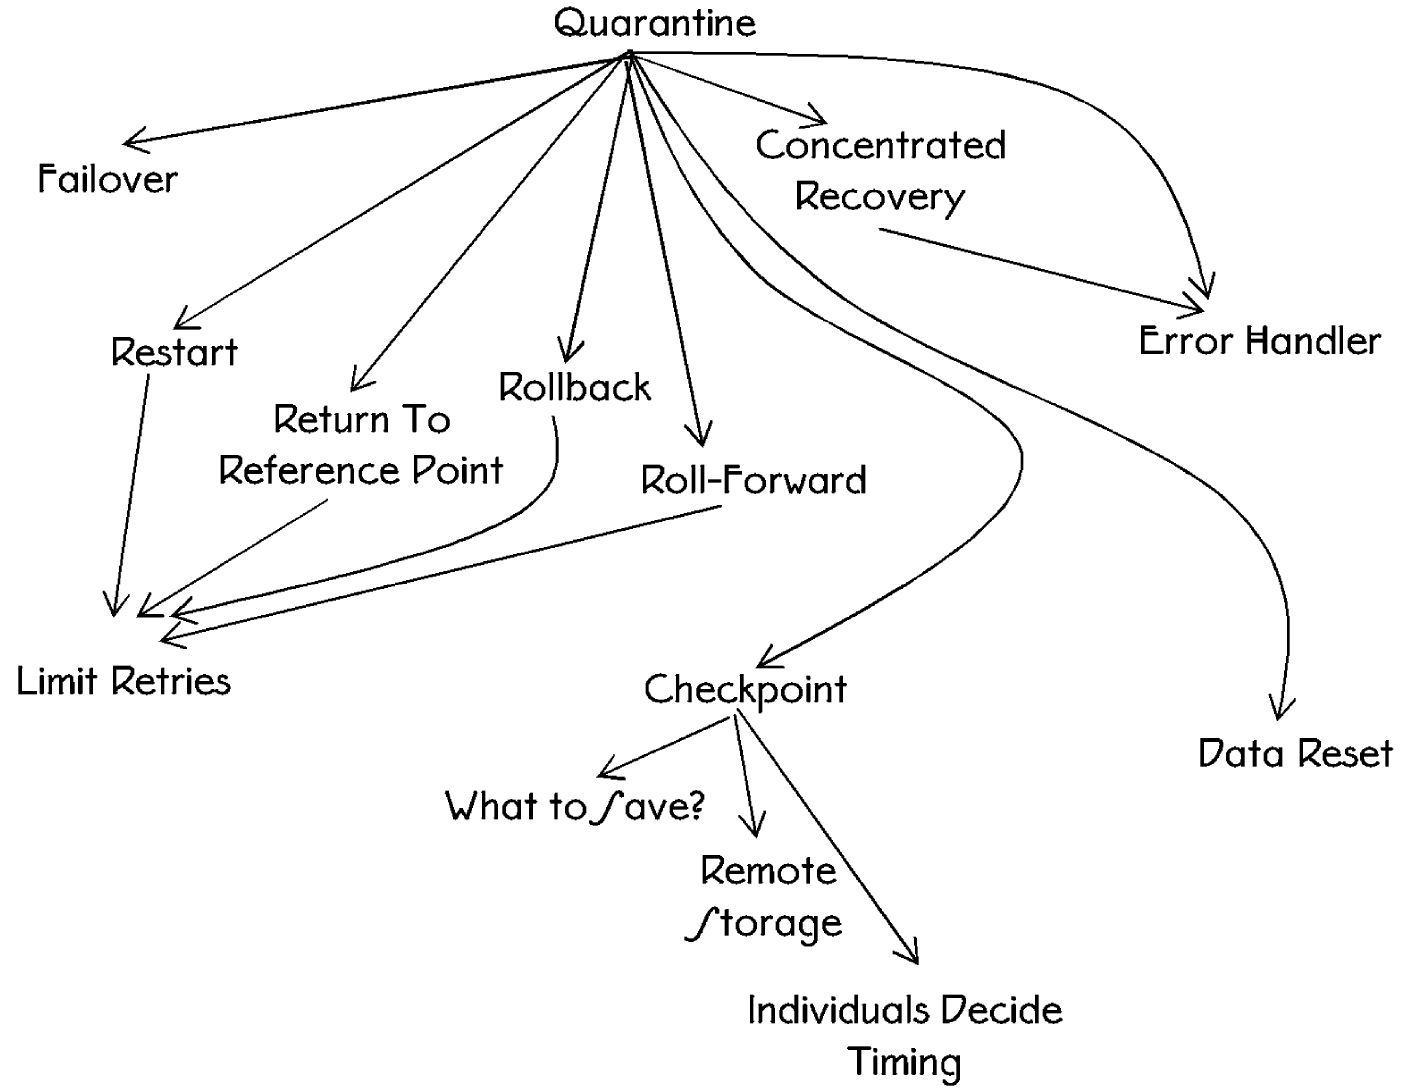
\includegraphics[width=\textwidth]{content/faulttolerance/images/RecoveryPatterns_Dependency.JPG}
	\caption{RecoveryPatterns Dependency}
\end{figure}


\subsubsection*{Error Recovery Patterns - Buch}

\begin{figure}[H]
	\centering
	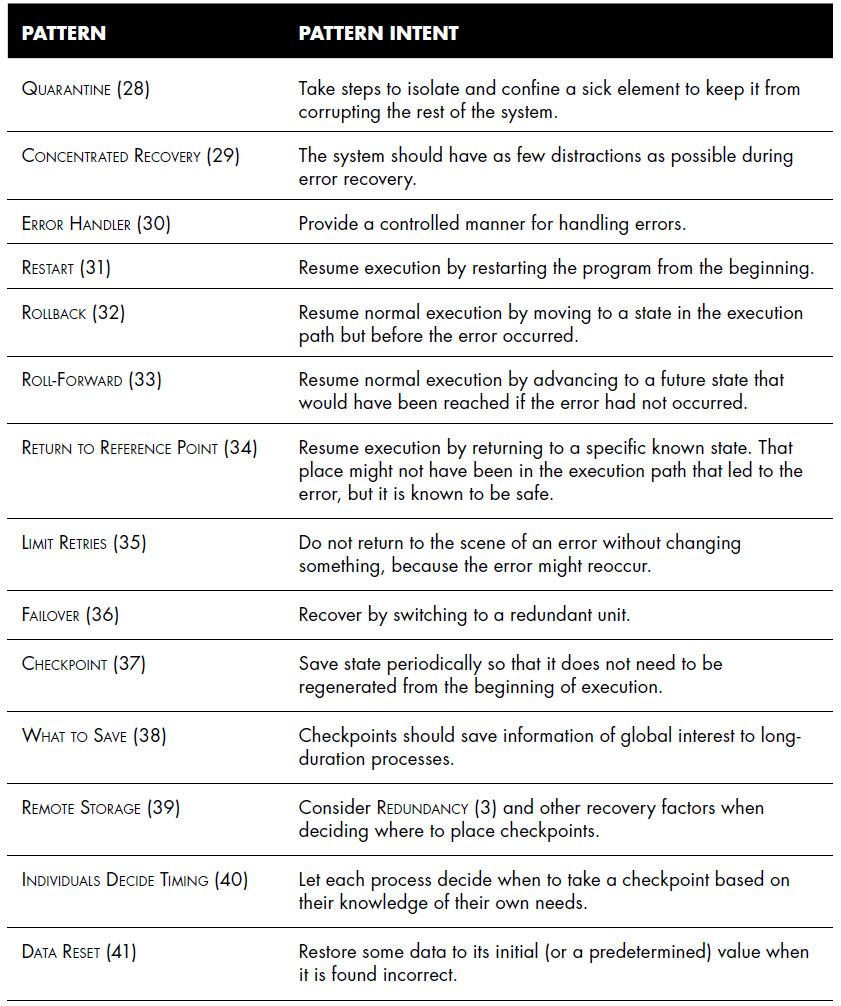
\includegraphics[width=\textwidth]{content/faulttolerance/images/RecoveryPatterns.JPG}
	\caption{RecoveryPatterns}
\end{figure}


\subsubsection*{Prüfungsfragen}

\begin{itemize}
	\item Erklären Sie den unterschied zwischen Error Detection und Error Recovery
	\item Was ist das Ziel, wenn ein Error Handler ``zum Einsatz'' kommt?
\end{itemize}

